% Section content template for individual Educative lessons
% This file contains the actual content for a specific section
% Generated from Educative API section content

% Section: Class Diagram for the Vending Machine
% Section ID: 5373748763164672
% Section Slug: class-diagram-for-the-vending-machine
% Generated: 2025-12-11T20:26:17.904924

In this lesson, we use a bottom-up approach to identify and design the classes and interfaces for our vending machine system. The focus is on clear responsibility separation, applying the State design pattern, and modeling relationships that reflect real-world constraints. Let 's explore each component and how they work together to realize our requirements.

\subsection{Components of a vending machine}\label{majDah7EZR35FHwR70wHB}
\\
As mentioned, we should design the vending machine using a bottom-up approach.

\subsubsection{State pattern and state}\label{8-83uQjwRojgfNpsMYQcD}
\\
We use the State design pattern to manage the vending machine's changing behavior depending on its current mode. This pattern encapsulates the machine's different operational ``states'' as separate classes, each handling user actions in its own way.
\\
\paragraph{State interface}\label{kmZNwcRcsZSf6OeCXIj6s}
\\
We define a \texttt{State} interface (or abstract base class), which exposes the two main user-facing actions:

\begin{itemize}
\item
\protect\phantomsection\label{etQaKl3SmdqgEXSrWdQvj}
\textbf{\texttt{insertMoney(amount)}:} For inserting cash into the machine.
\item
\protect\phantomsection\label{A9ZU1jHBdH-amySgKR1Q9}
\textbf{\texttt{selectProduct(rackNumber)}:} For selecting a product to purchase.
\end{itemize}
\\
The machine is in exactly one of the following three concrete states at any moment. Each state provides its logic for these actions:

\begin{enumerate}
\item
\protect\phantomsection\label{5PvAVXmX5jSML7EurrMjR}
\textbf{\texttt{NoMoneyInsertedState}}

\begin{enumerate}
\item
\textbf{\texttt{insertMoney}:} Records the inserted amount and transitions the machine to the \texttt{MoneyInsertedState}.
\item
\textbf{\texttt{selectProduct}:} Rejects the request with a message (e.g., ``Please insert money first'').
\end{enumerate}
\item
\protect\phantomsection\label{r1dhO9ZqJTEp8kVgfl4t2}
\textbf{\texttt{MoneyInsertedState}}

\begin{enumerate}
\item
\textbf{\texttt{insertMoney}:} Adds to the current balance.
\item
\textbf{\texttt{selectProduct}:}

\begin{enumerate}
\item
Checks if the selected product is available and compares the current balance to the product price:

\begin{enumerate}
\item
\textbf{Underpaid:} Returns all inserted money and resets to \texttt{NoMoneyInsertedState}.
\item
\textbf{Exact payment:} Dispenses the selected product and transitions to \texttt{DispenseState}.
\item
\textbf{Overpayment:} Dispenses the product, returns the change, and transitions to \texttt{DispenseState}.
\end{enumerate}
\end{enumerate}
\end{enumerate}
\item
\protect\phantomsection\label{qmxNb4aKE3xbjWXRLcNYe}
\textbf{\texttt{DispenseState}}

\begin{enumerate}
\item
\textbf{\texttt{insertMoney}:} Does not accept any new actions; prompts the user to wait (e.g., ``Please wait, dispensing in progress\ldots'').
\item
\textbf{\texttt{selectProduct}:} Same as above; defers all actions while dispensing.
\item
After the product (and any change) is delivered, the machine resets to \texttt{NoMoneyInsertedState}.
\end{enumerate}
\end{enumerate}
\\
Every state implements some functions, as shown below:

\begin{figure}[htbp]
 \centering
 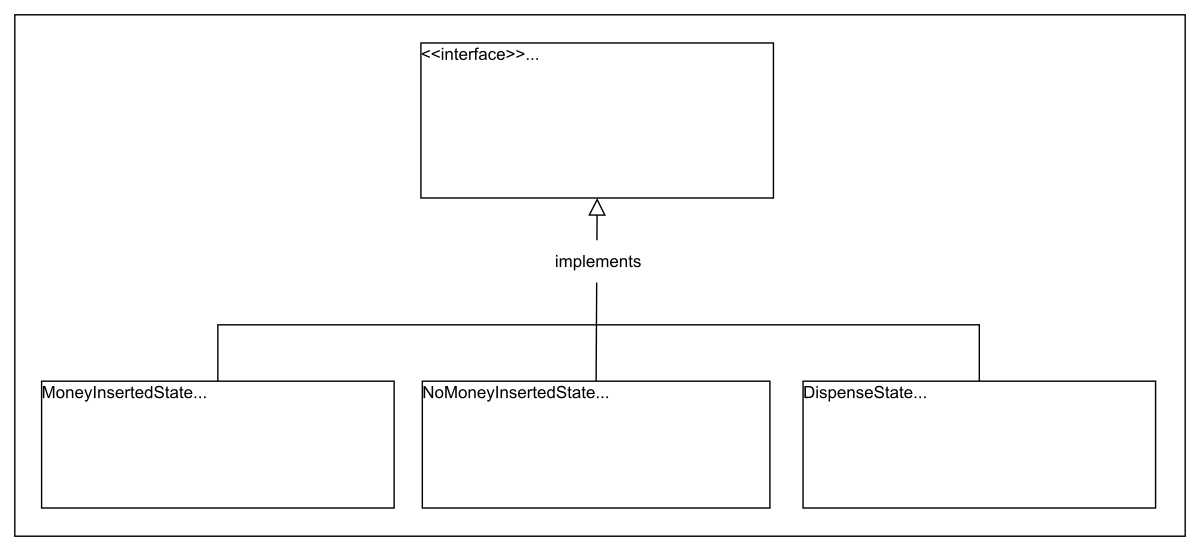
\includegraphics[width=0.5\textwidth]{Images/chapter_11/section_5373748763164672/5401838068039680.png}
 \caption{The class diagram of the State interface and its subclasses}
\end{figure}

\textbf{R2:} The vending machine can be in one of these three states:

\begin{itemize}
\tightlist
\item
There is no money inserted into the machine.
\item
Money is inserted into the machine.
\item
The machine gives out the product.
\end{itemize}
\\
\textbf{R6:} Users can insert money (cash) into the machine; the system should accept, validate, and count the amount.
\\
\textbf{R7:} The system should be able to calculate the money inserted into the machine.
\\
\textbf{R8:} The system should check whether the user inserted the exact amount required for the specific product into the machine.
\\
\textbf{R9:} If the amount exceeds the product price, the system should change back to the user and dispense the product.
\\
\textbf{R10:} If the amount exceeds the product price, the system should display an error message and return the money.

\begin{quote}
\textbf{Note:} According to the implementation of the State design pattern, all functions will be available in each state. However, not every function must have a meaningful definition for that particular state.
\end{quote}
\subsubsection{Product}\label{VIQvEiX-jL-0z8CIN515k}
\\
The \texttt{Product} class contains the details of a particular product available in the vending machine. Each product has a \texttt{name}, \texttt{id}, \texttt{price}, and its \texttt{type} associated with it as presented below:

\begin{figure}[htbp]
 \centering
 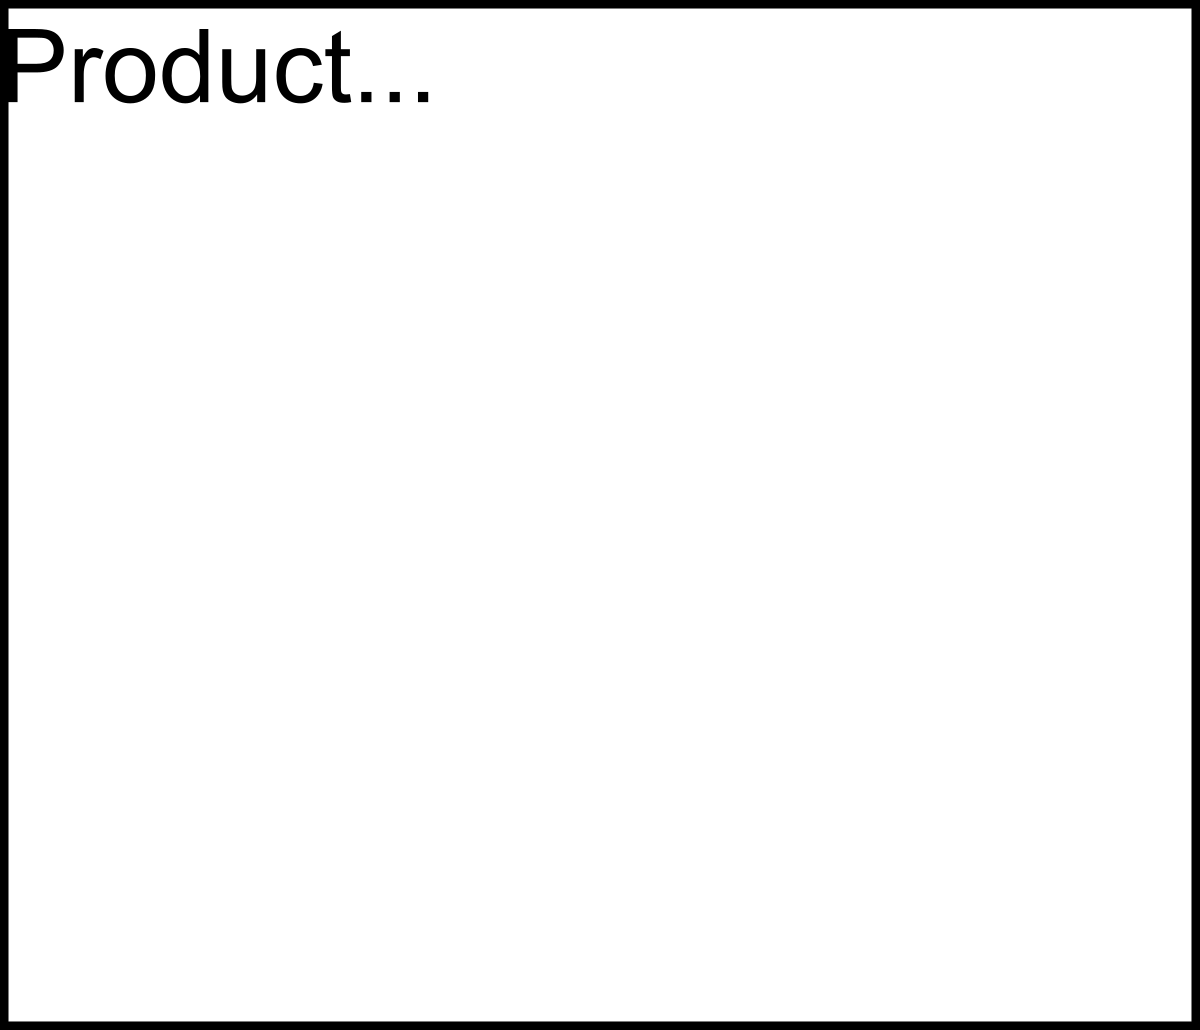
\includegraphics[width=0.5\textwidth]{Images/chapter_11/section_5373748763164672/4759775164497920.png}
 \caption{The class diagram of the Product class}
\end{figure}

\textbf{R1:} The vending machine stores and manages different types of products, each placed at a unique slot within the machine.
\\
\textbf{R5:} The system should allow the users to select a product they want to purchase from the machine by specifying the rack number.

\subsubsection{Rack}\label{Nij3RcvXn2wXyYmgfcAr3}
\\
The \texttt{Rack} class is used to identify the location of the products in the vending machine. Every rack has a specific \texttt{rackNumber} as an identifier, the \texttt{product} it has, and the \texttt{quantity} of the product. The class representation is provided below:

\begin{figure}[htbp]
 \centering
 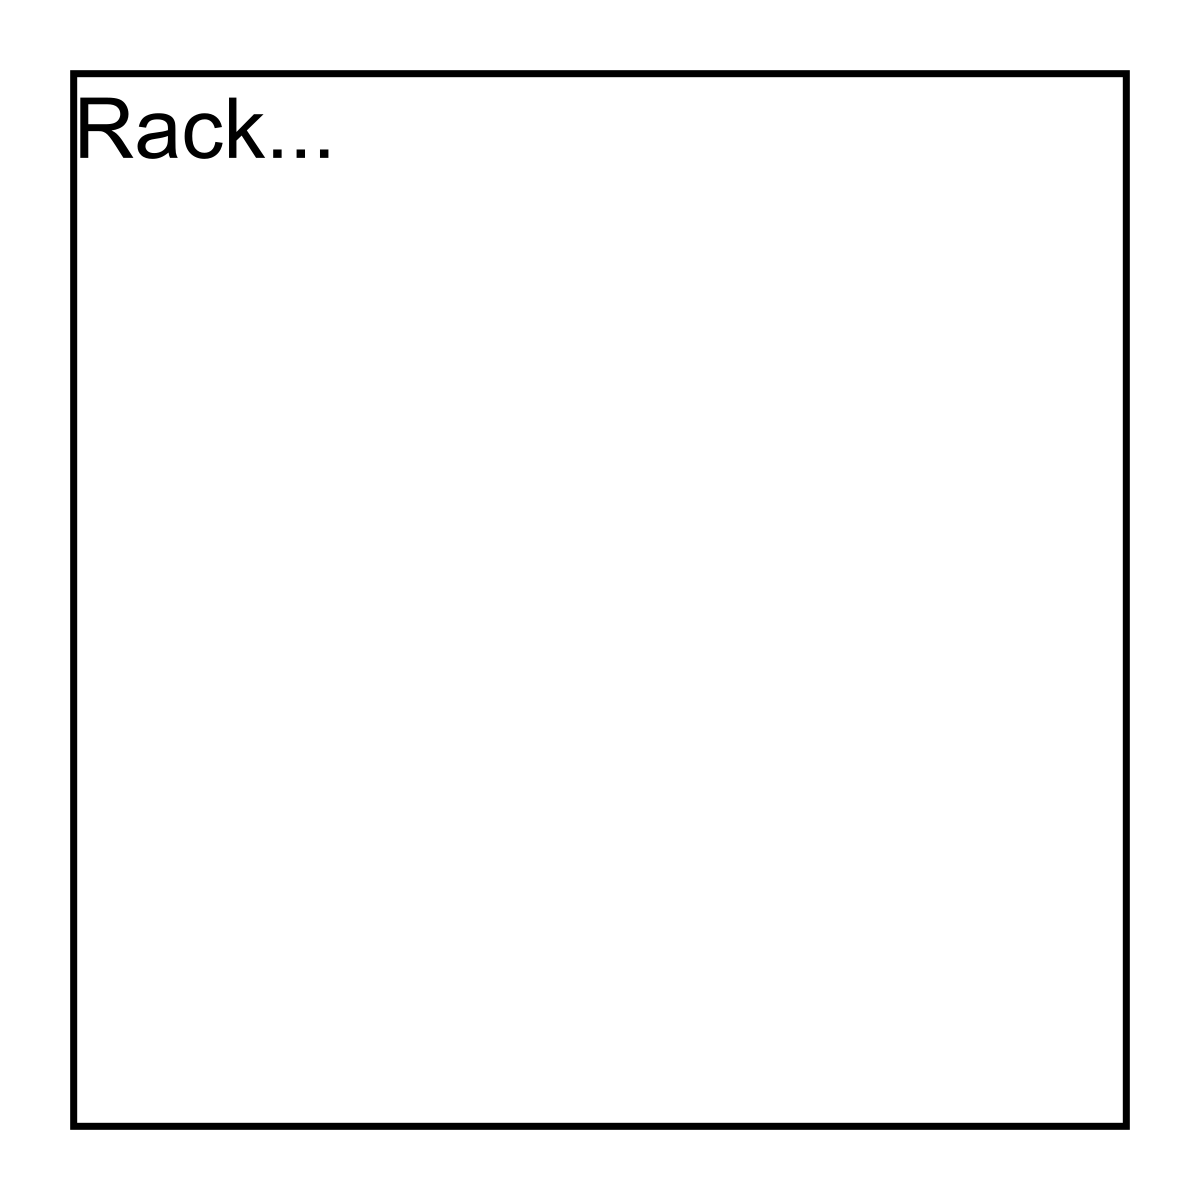
\includegraphics[width=0.5\textwidth]{Images/chapter_11/section_5373748763164672/6145975100768256.png}
 \caption{The class diagram of the Rack class}
\end{figure}

\textbf{R1:} The vending machine stores and manages different types of products, each placed at a unique slot within the machine.
\\
\textbf{R5:} The system should allow the users to select a product they want to purchase from the machine by specifying the rack number.

\subsubsection{Inventory}\label{3MOigKej2PxKoT0r3sMOy}
\\
The \texttt{Inventory} class manages a collection of racks inside the vending machine. Internally , it keeps a map from each rack number to its corresponding \texttt{Rack} object. It provides three core operations:

\begin{enumerate}
\item
\protect\phantomsection\label{zdSSCkYOs2t9DDQadLuK0}
addRack(Rack\ rack): Register a new rack in the machine.
\item
\protect\phantomsection\label{Q35CPQXp6sh0Vt9t3Xbf1}
getRack(int\ rackNumber): Look up and return the rack for the given position (or \texttt{null} if none exists).
\item
\protect\phantomsection\label{-0Ta_eQ5QOHo7LAbyBqI6}
\texttt{allRacks()}: Retrieve every rack currently in the machine.
\end{enumerate}
\\
This design makes it easy to load, dispense, and inspect products by rack number without exposing any lower-level list or count fields.
\\
The class representation is provided below:

\begin{figure}[htbp]
 \centering
 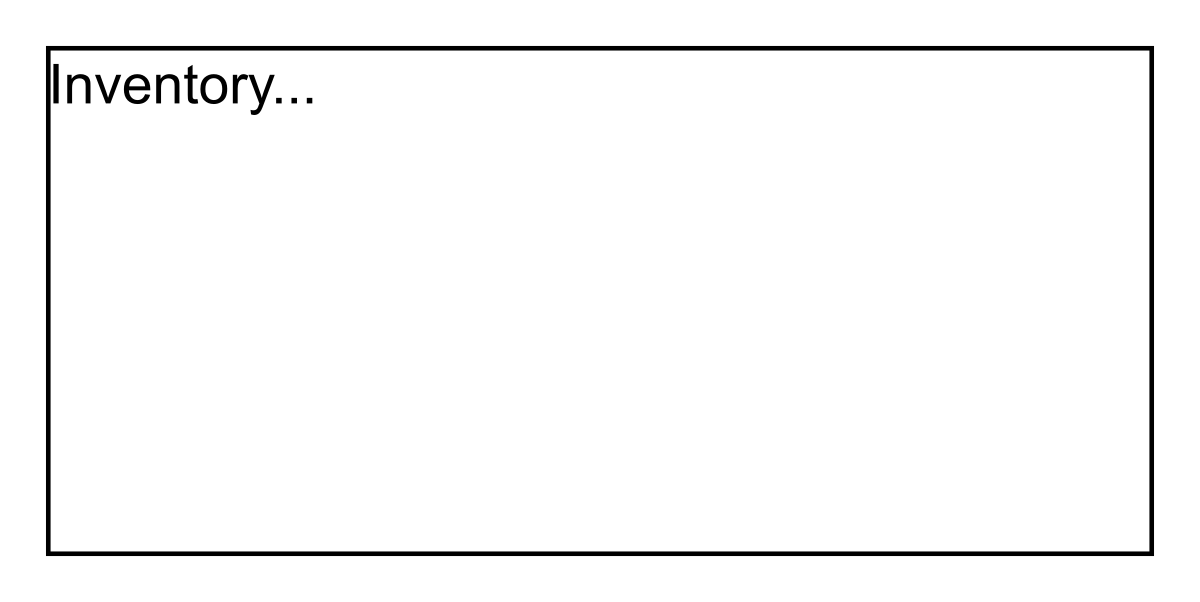
\includegraphics[width=0.5\textwidth]{Images/chapter_11/section_5373748763164672/6218430041423872.png}
 \caption{The class diagram of the Inventory class}
\end{figure}

\textbf{R1:} The vending machine stores and manages different types of products, each placed at a unique slot within the machine.
\\
\textbf{R4:} The admin can add or remove new products to the machine.

\subsubsection{VendingMachine}\label{XRp1wiYZ7peDsR66tZrTr}
\\
The \texttt{VendingMachine} class is the central context in our State pattern design. It is a Singleton (only one instance exists) and holds:

\begin{itemize}
\item
\protect\phantomsection\label{rbBmui-UTqAhtxmiRACZb}
Current state (\texttt{State})
\item
\protect\phantomsection\label{SyRa3UgO7WsjhEMqaJYs4}
Current balance (the total cash inserted so far)
\item
\protect\phantomsection\label{SeAXKneffMTKwfqCjuLLq}
Inventory (the collection of racks and their contents)
\end{itemize}
\\
All external calls---\texttt{insertMoney(amount)} and \texttt{selectProduct(rackNumber)}---simply delegate to whatever \texttt{State} object is active. The machine itself handles:

\begin{enumerate}
\item
\protect\phantomsection\label{lrbydbmb1PDPwYjaaldpg}
State transitions (No money → Money inserted → Dispense → No money)
\item
\protect\phantomsection\label{VJZRPx2FFMAogKwcag4tb}
Actual dispensing/refunding logic (once the state says it's ``OK'' to dispense)
\item
\protect\phantomsection\label{Wj-sYvwOKTn3DCrpe9QZB}
Admin operations (loading racks, collecting cash)---kept entirely outside the State interface.
\end{enumerate}
\\
By pushing only the two user actions into the State subclasses, and keeping everything else in the context, we get a clear separation of ``what changes when'' vs. ``how things actually happen.'' The class representation is provided below:

\begin{figure}[htbp]
 \centering
 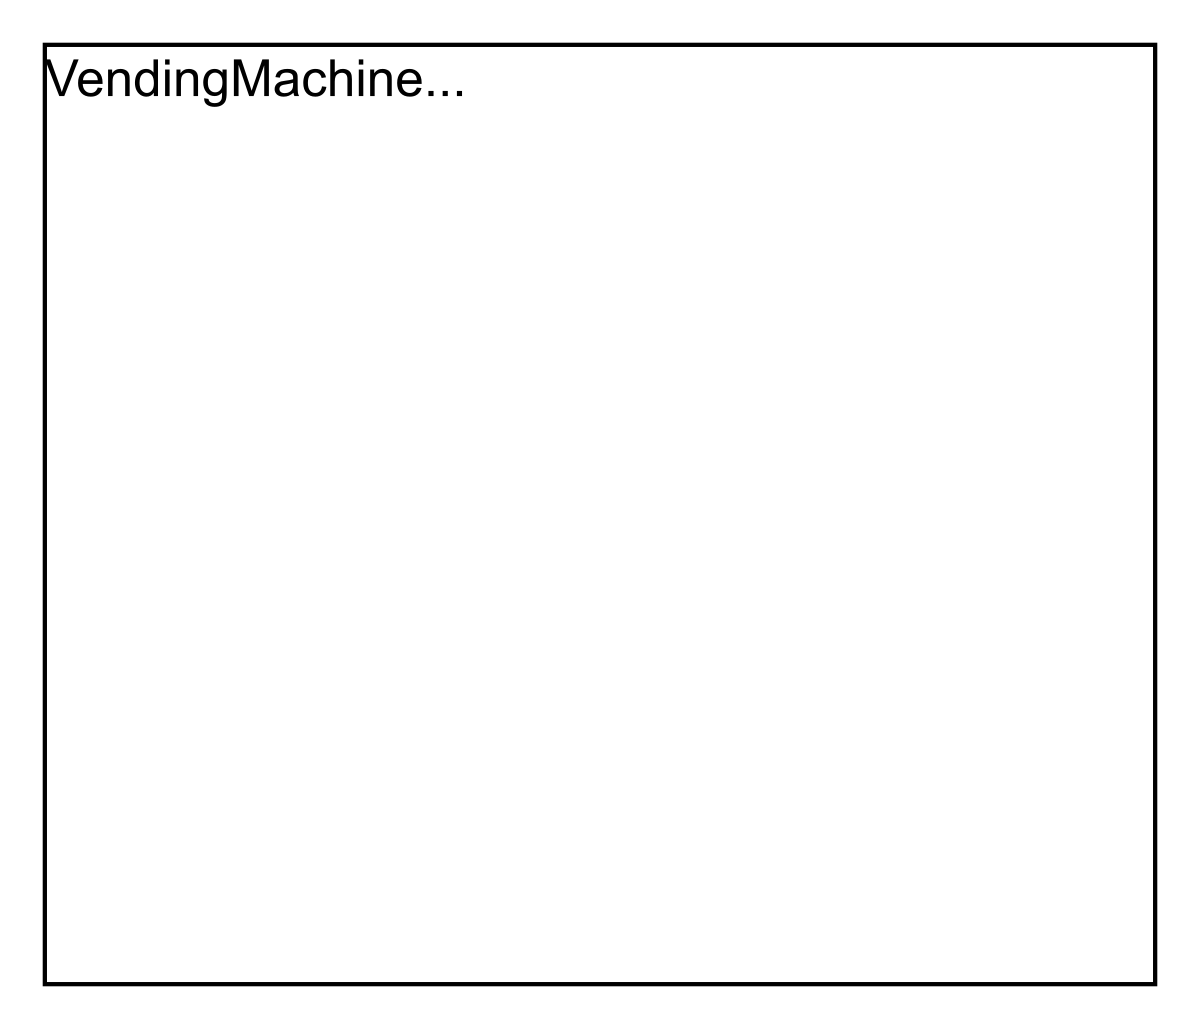
\includegraphics[width=0.5\textwidth]{Images/chapter_11/section_5373748763164672/6645290692902912.png}
 \caption{The class diagram of the VendingMachine class}
\end{figure}

\textbf{R2:} The vending machine can be in one of these three states:

\begin{itemize}
\tightlist
\item
\textbf{NoMoneyInsertedState:} There is no money inserted into the machine.
\item
\textbf{MoneyInsertedState:} Money is inserted into the machine.
\item
\textbf{DispenseState:} The machine gives out the product.
\end{itemize}
\\
\textbf{R5:} The system should allow the users to select a product they want to purchase from the machine by specifying the rack number.
\\
\textbf{R6:} Users can insert money (cash) into the machine.
\\
\textbf{R7:} The system should be able to calculate the money inserted into the machine.
\\
\textbf{R8:} The system should check whether the user has inserted the exact amount required for the specific product into the machine.
\\
\textbf{R9:} If the amount exceeds the product price, the system should change the user back and dispense the product.
\\
\textbf{R10:} If the amount exceeds the product price, the system should display an error message and return the money.

\subsubsection{Enumeration}\label{9g4kSHp8yR4-68u8PpAgH}
\\
The enumeration required to design the vending machine system is provided below:
\\
\paragraph{ProductType}\label{5AHqfjqp5z_g5nRL-hhgg}
\\
We need to create an enumeration to keep track of the type of product, whether it is chocolate, a snack, a beverage, or another type.

\begin{figure}[htbp]
 \centering
 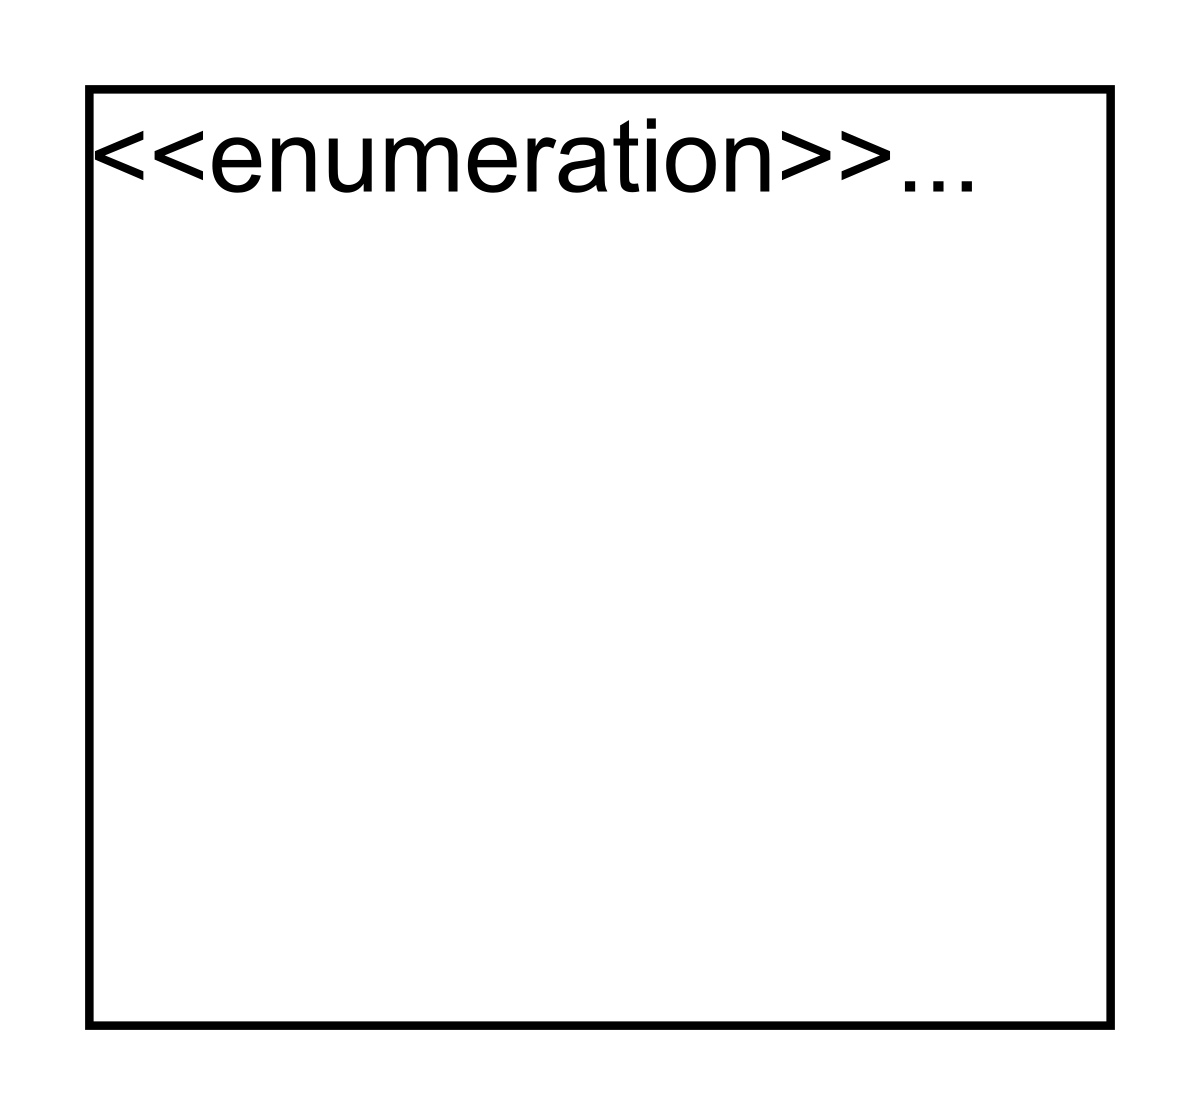
\includegraphics[width=0.5\textwidth]{Images/chapter_11/section_5373748763164672/6640089546227712.png}
 \caption{The ProductType enumeration}
\end{figure}

\subsection{Relationship between the classes}\label{pDu8qF2EMoAi9wYzMDnTy}
\\
Now, we'll discuss the relationships between the classes we have defined above in our vending machine.

\subsubsection{Composition}\label{urRAEwavtPPEaL8sSSAJl}
\\
We use composition to show strong ``owns‐a'' relationships wherever one object cannot meaningfully exist without its container:

\begin{enumerate}
\item
\protect\phantomsection\label{15cCMIWHRNX1Et9F6_NMJ}
\texttt{VendingMachine} is composed of \texttt{Inventory}.

\begin{enumerate}
\item
The machine contains exactly one \texttt{Inventory} instance.
\item
If the machine is torn down, its inventory goes with it.
\end{enumerate}
\item
\protect\phantomsection\label{KkpexBgW4GLjs6fwR1BuD}
\texttt{Inventory} is composed of \texttt{Rack}.

\begin{enumerate}
\item
The inventory manages a collection of racks (one per slot).
\item
Each \texttt{Rack} lives and dies inside its \texttt{Inventory}.
\end{enumerate}
\item
\protect\phantomsection\label{y4cQYVQxiiO7Ilb2uMaUs}
\texttt{Rack} is composed of \texttt{Product}.

\begin{enumerate}
\item
A rack always holds a specific \texttt{Product} (plus a quantity).
\item
You cannot have a rack without knowing what product it contains.
\end{enumerate}
\end{enumerate}
\\
Visually, each arrow is a filled diamond at the container end:

\begin{figure}[htbp]
 \centering
 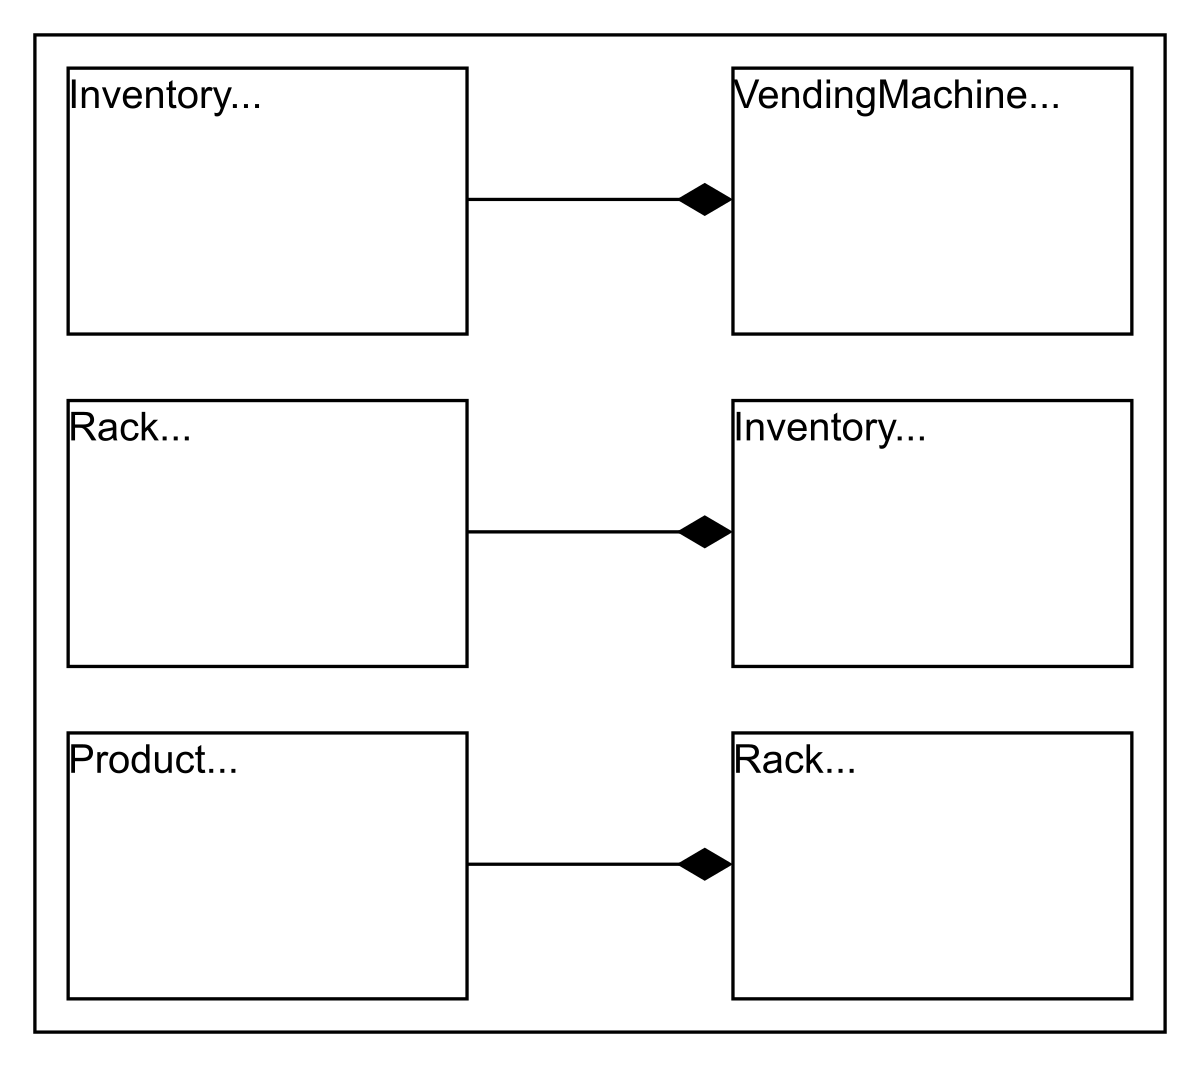
\includegraphics[width=0.5\textwidth]{Images/chapter_11/section_5373748763164672/5436630314647552.png}
 \caption{The composition relationship between classes}
\end{figure}

This structure ensures that:

\begin{itemize}
\item
\protect\phantomsection\label{agZ09xZjdCUbNKnj9RX7w}
Only the \texttt{VendingMachine} can create or destroy the entire \texttt{Inventory}.
\item
\protect\phantomsection\label{A0UFlCSiLwGpCiKvAz11k}
Only \texttt{Inventory} can add or remove \texttt{Rack} objects.
\item
\protect\phantomsection\label{0Z0anCYjn54JUJ_M9vS5Q}
Only each \texttt{Rack} can load or unload its own \texttt{Product}.
\end{itemize}
\\
By modeling these as compositions, we clearly express ownership and the life cycle dependencies among our core classes.

\subsubsection{Aggregation}\label{EoG19rBPkEStqV5zFfM4P}
\\
The class diagram has the following aggregation relationships:

\begin{itemize}
\item
\protect\phantomsection\label{UWhD7FupLAPt85y4kKsq3}
The \texttt{VendingMachine} class contains the \texttt{State} interface.
\end{itemize}

\begin{figure}[htbp]
 \centering
 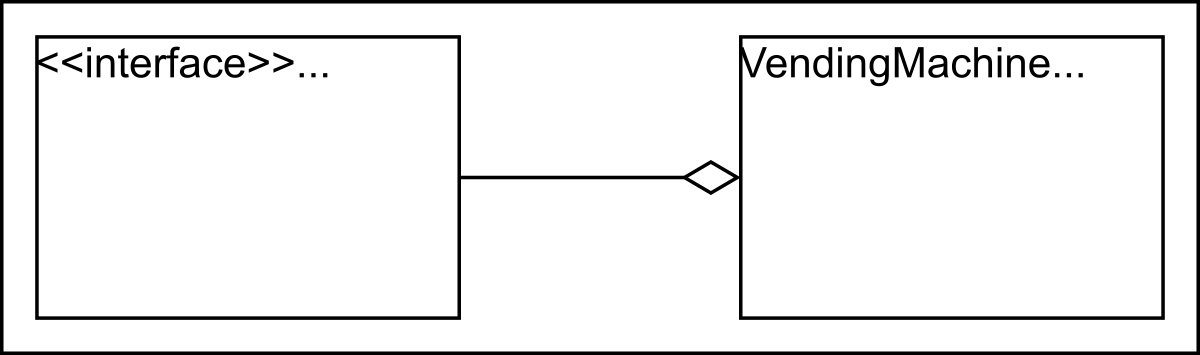
\includegraphics[width=0.5\textwidth]{Images/chapter_11/section_5373748763164672/4900957366517760.png}
 \caption{The aggregation relationship between classes}
\end{figure}

\subsubsection{Association}\label{IpT14eeOqN3yfVm6AEKyx}
\\
Besides the strong ownership shown by our composition arrows, we also have simple ``uses-a'' links between classes. In UML, these are unfilled‐arrow or line associations with no diamond:

\begin{itemize}
\item
\protect\phantomsection\label{YJAIr5X1V1Bw8wWEPpmgo}
\texttt{VendingMachine} \textbf{→} \texttt{Inventory}\\
The machine holds one \texttt{Inventory} object and calls its lookup methods to find racks.
\item
\protect\phantomsection\label{BpiTfwUrmhA23jDNjTIPq}
\texttt{VendingMachine} \textbf{→} \texttt{State}\\
The machine keeps a reference to its current \texttt{State} (No money, Money inserted, or Dispense) and delegates \texttt{insertMoney}/\texttt{selectProduct} to it.
\item
\protect\phantomsection\label{QyuGImYrNo6Y3swsvA1no}
\texttt{Inventory} \textbf{→} \texttt{Rack}\\
Internally, \texttt{Inventory} stores many \texttt{Rack} instances (one per slot) and looks them up by rack number.
\item
\protect\phantomsection\label{b9_2ft0zptUKtUJ8Hod0k}
\texttt{Rack} \textbf{→} \texttt{Product}\\
Each rack refers to exactly one \texttt{Product} (plus a quantity) when loaded.
\end{itemize}
\\
Visually, you'd draw each of these as a straight line (or arrow) from the ``user'' class to the ``used'' class, with multiplicities as needed.

\begin{figure}[htbp]
 \centering
 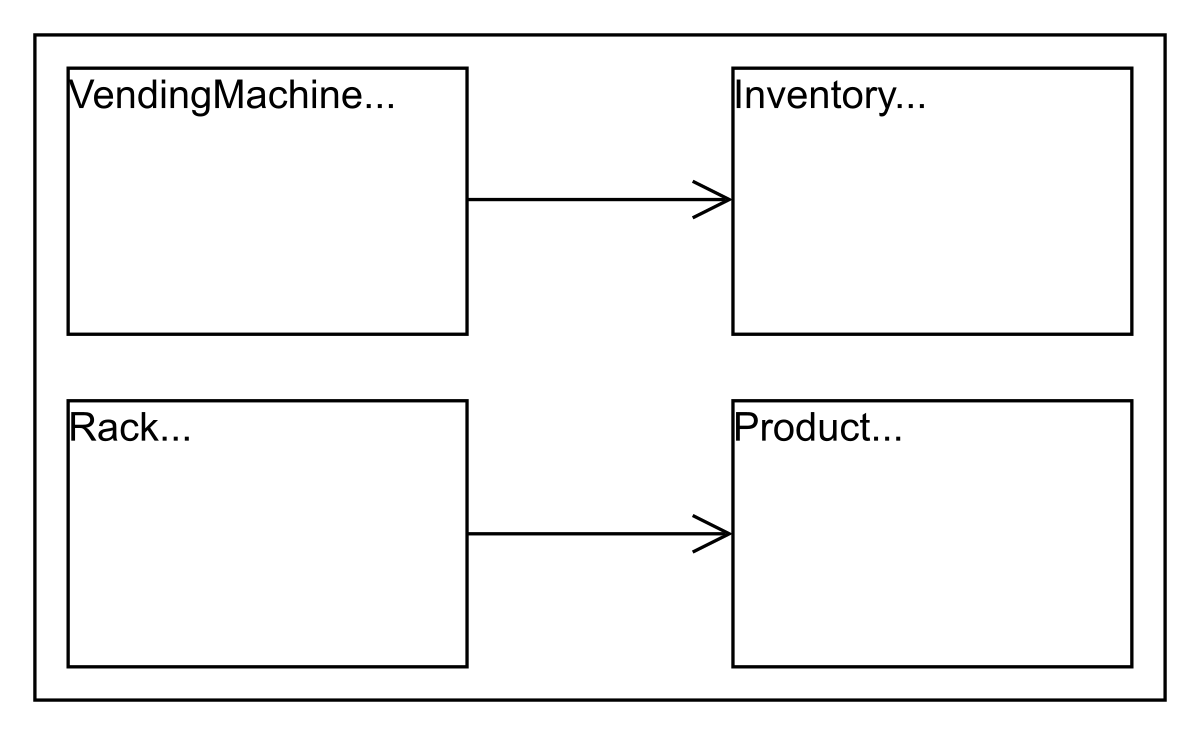
\includegraphics[width=0.5\textwidth]{Images/chapter_11/section_5373748763164672/6476507730804736.png}
 \caption{The association relationship between classes}
\end{figure}

\subsubsection{Inheritance}\label{9mURtb02Vh8rpmisC5BdE}
\\
Inheritance in object-oriented design allows classes to share contracts (interfaces/abstract classes) or behaviors (concrete classes). Our three concrete state classes---\texttt{NoMoneyInsertedState}, \texttt{MoneyInsertedState}, and \texttt{DispenseState}---all implement the common \texttt{State} interface. Referring to the UML under the ``State pattern and State'' section, this is shown with a solid line and a hollow triangle pointing to the superclass or the \texttt{State} interface.

\begin{itemize}
\item
\protect\phantomsection\label{KokdFMtoh-ezkdCtdjCVo}
\texttt{State} defines the two key operations (\texttt{insertMoney} and \texttt{selectProduct}) without prescribing how they work.
\item
\protect\phantomsection\label{6UUl_uxNo187ugcC3yy7e}
Each concrete state class inherits that contract and provides its own behavior for those methods, according to the vending machine's current mode.
\end{itemize}
\\
This arrangement lets the \texttt{VendingMachine} treat all states uniformly (polymorphism), while each subclass specializes the response to user actions exactly as its particular state requires.
\begin{quote}
\textbf{Note:} We have already discussed this inheritance relationship between classes in the component section above.
\end{quote}
\subsection{Class diagram for the vending machine}\label{6_5PQWr0sSZK4UjCVH12v}
\\
This section outlines the multiplicity (cardinality) relationships between the main classes in our Vending Machine system. We explain the allowed number of instances on each side for each relationship and the real-world or design rationale behind the connection. Understanding these relationships is key to modeling how different entities interact and collaborate to support key workflows in the system.

\begin{center}
\begin{tabular}{|p{0.20\linewidth}|p{0.20\linewidth}|p{0.15\linewidth}|p{0.40\linewidth}|}
\hline
\textbf{Source} & \textbf{Target} & \textbf{Multiplicity} & \textbf{Reason} \\
\hline
VendingMachine & Inventory & 1 --- 1 & Each VendingMachine has exactly one Inventory, which manages all racks and products. The inventory is tightly coupled and cannot exist without its machine. \\
\hline
Inventory & Rack & 1 --- 1..* & Each Inventory manages one or more Rack objects. A machine must have at least one rack to function, and can have many racks for different products. \\
\hline
Rack & Product & 1 --- 1 & Each Rack holds exactly one Product at a time (plus quantity) and is designed for one product type throughout its life cycle. \\
\hline
VendingMachine & State & 1 --- 1 (current), 1 --- 3 (total) & The VendingMachine references exactly one current State at runtime, but owns all three possible state instances internally (State Pattern). \\
\hline
State & Concrete State (NoMoneyInsertedState, MoneyInsertedState, DispenseState) & 1 --- 3 (implements) & The State interface is implemented by three concrete classes, representing the possible operational states of the vending machine. \\
\hline
\end{tabular}
\end{center}

Here is the complete class diagram for our vending machine:

\begin{figure}[htbp]
 \centering
 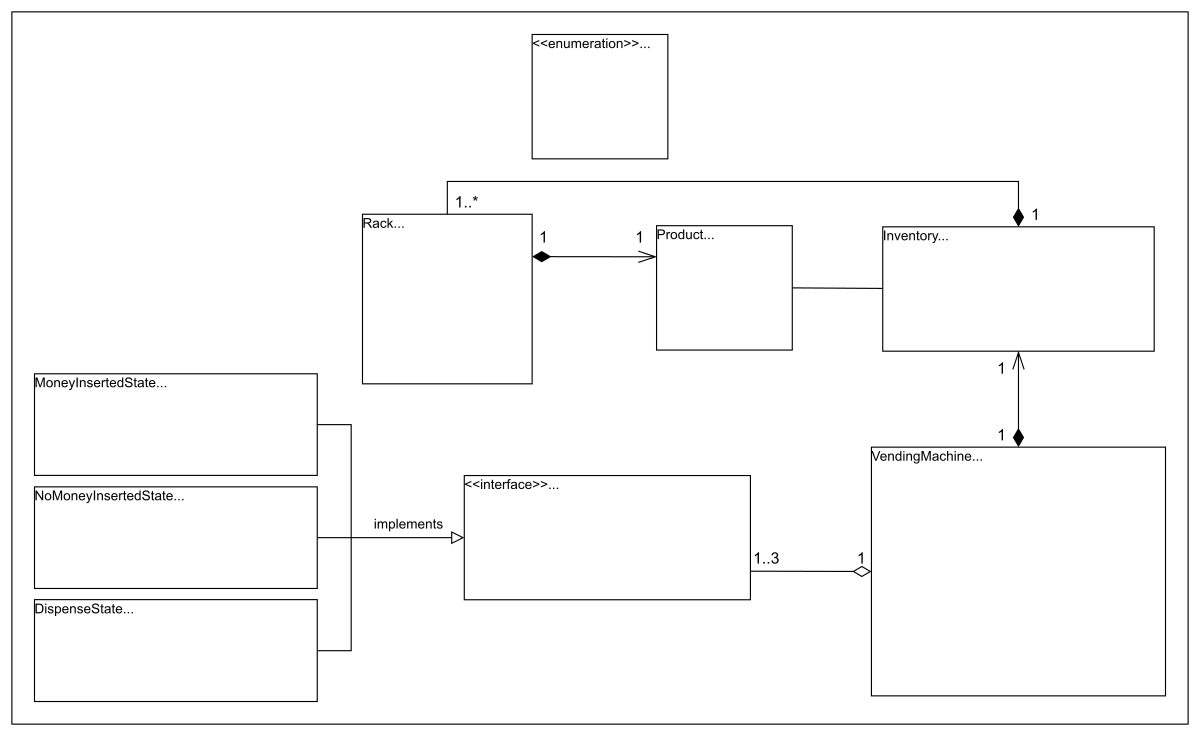
\includegraphics[width=0.5\textwidth]{Images/chapter_11/section_5373748763164672/5575872416186368.png}
 \caption{The class diagram of the vending machine}
\end{figure}

\subsection{Design pattern}\label{oIdKXBdrCOuV_2vRJjx1M}
\\
We apply the \emph{State pattern} because the vending machine's behavior changes depending on its current mode. At runtime, it lives in exactly one of three states:

\begin{itemize}
\item
``No money'' state
\item
``Money inserted'' state
\item
``Dispense'' state
\end{itemize}
\\
Each state exposes the same two operations (\texttt{insertMoney} and \texttt{selectProduct}), but implements them differently---rejecting selections when no cash is in, accumulating balance when money is inserted, validating price vs. balance when a product is chosen, or blocking all input while dispensing.
\begin{quote}
By encapsulating each behavior in its own state class, we avoid large \texttt{if/else} or \texttt{switch} statements inside the machine, making the code easier to maintain and extend (e.g., adding a ``Maintenance'' or ``OutOfOrder'' state in the future without touching existing logic).
\end{quote}
\subsection{AI-powered trainer}\label{Ux6etZx-ysj8rv-WYHZ2f}
\\
At this stage, everything should be clear. If you encounter any confusion or ambiguity, feel free to utilize the interactive AI-enabled widget below to seek clarification. This tool is designed to help you strengthen your understanding of the concepts.

\begin{figure}[htbp]
 \centering
 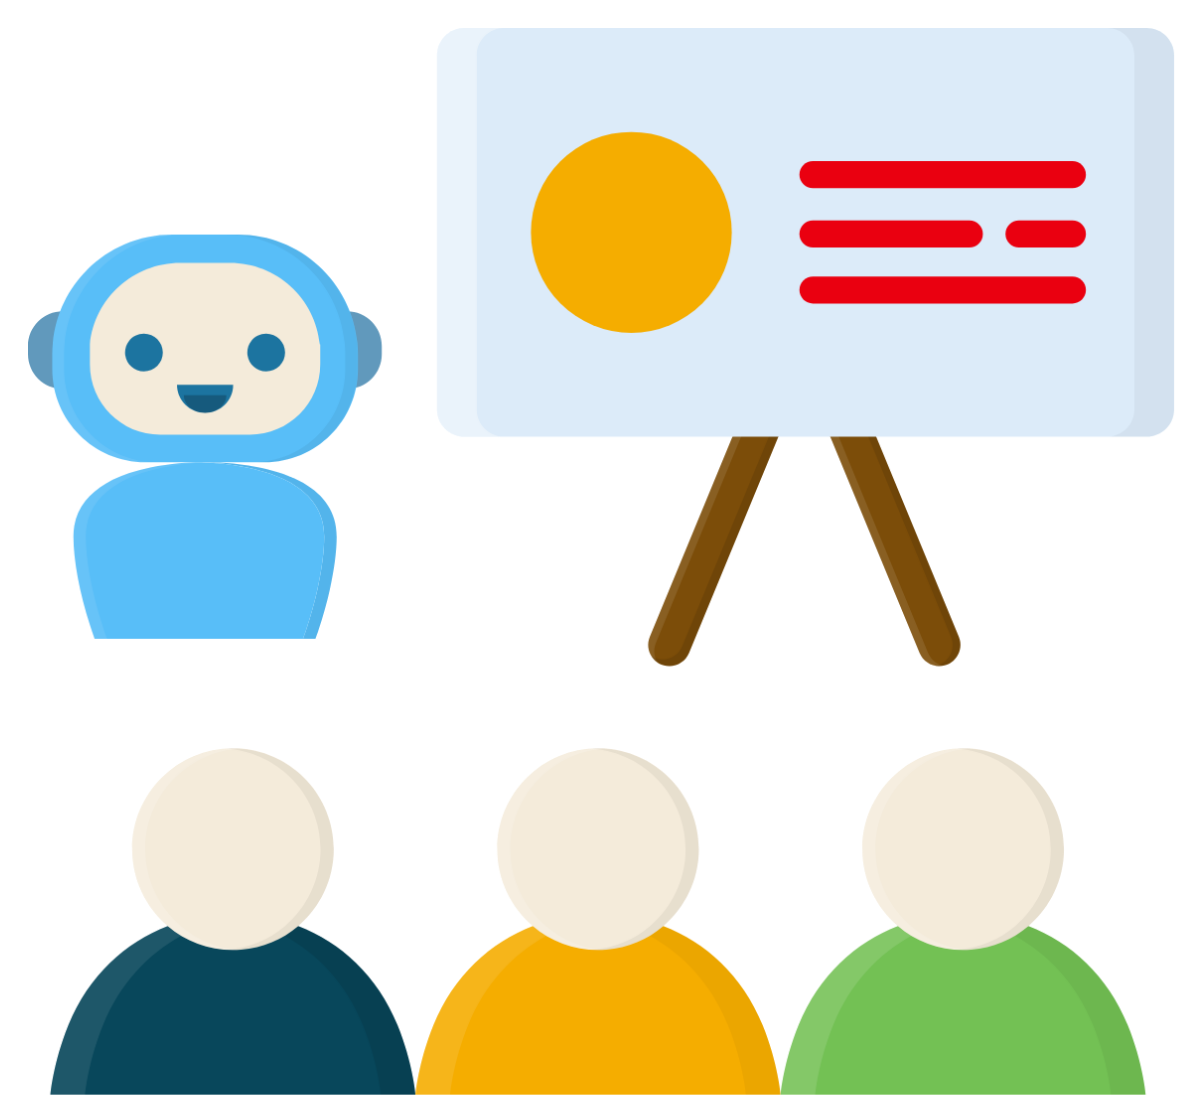
\includegraphics[width=0.15\textwidth]{Images/chapter_11/section_5373748763164672/6345713003659264.png}
 
\end{figure}

\subsection{Additional requirements}\label{cUgoLTXGI3n_corzOTXPc}
\\
The interviewer can introduce some additional requirements in the vending machine, or they can ask some follow-up questions. Let 's see some examples of additional requirements:
\\
\textbf{Refund/Cancel:} The vending machine should have the option to cancel the operation. In that case, the customers will get a refund. The class diagram provided below shows the refund functionality in all states:

\begin{figure}[htbp]
 \centering
 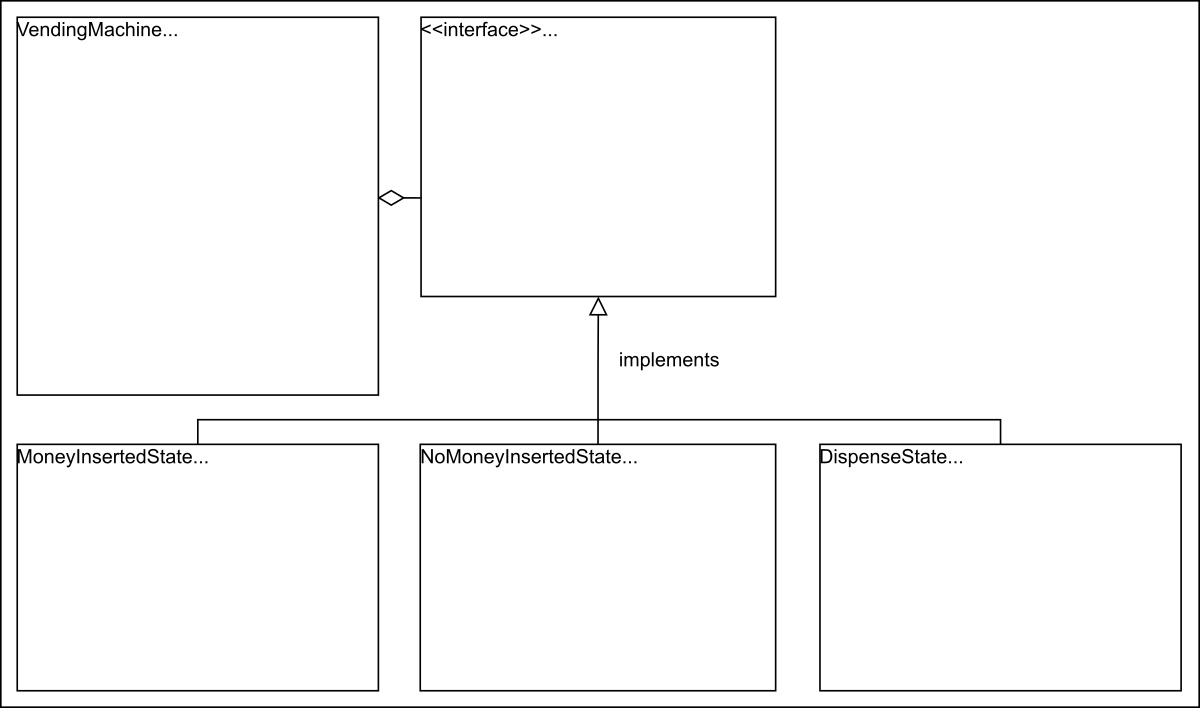
\includegraphics[width=0.5\textwidth]{Images/chapter_11/section_5373748763164672/6149052483895296.png}
 \caption{Modified class diagram of the vending machine}
\end{figure}

In the class diagram above, we can see a function,\ refundFullMoney(), in all states, which is used to refund the full money. Here is the definition of the \texttt{refundFullMoney()} function according to each state:

\begin{itemize}
\item
\protect\phantomsection\label{sy7wQ6S4uVA8FurUFsgC-}
\texttt{NoMoneyInsertedState}: In this state, the refundFullMoney()\ function throws an exception or warning, ``Please insert some cash first,'' because we have not inserted any money yet.
\item
\protect\phantomsection\label{yniAAtEl2wHa7UgVBfuOD}
\texttt{MoneyInsertedState}: In this state, we know the customer inserted the cash because we shifted the vending machine's state from \texttt{NoMoneyInsertedState} to \texttt{MoneyInsertedState}. If the customer uses the refund option, the \texttt{refundFullMoney()} function will be called and return the full amount to the change tray.
\item
\protect\phantomsection\label{d-C8AUEnna4YZDmcIIXbN}
\texttt{DispenseState}: In this state, the \texttt{refundFullMoney()} function is blocked. If the customer uses the refund option, the system does nothing. This is because the customer has selected a product, and the vending machine is in the dispense state.
\end{itemize}
\\
We have completed the class diagram of a vending machine according to the requirements. In the next lesson, let's design the activity diagram of the vending machine.

% End of section content